\documentclass{article}

\usepackage[T1]{fontenc}    %Schriftart des Dokumentes
\usepackage[ngerman]{babel} %Dokumentensprache, hier Deutsch
\usepackage{amsmath, amssymb, stmaryrd} %mathematische Schriftzeichen
\usepackage{graphicx} %Einfügen von Grafiken
\usepackage{wrapfig}
\usepackage{bm}
\usepackage{subfig}
\usepackage{newclude}
\usepackage{pdfpages}
\usepackage{hyperref}
\hypersetup{
    colorlinks,
    citecolor=black,
    filecolor=black,
    linkcolor=black,
    urlcolor=black
}

\makeatletter
\newcommand\invisiblesection[1]{%
  \refstepcounter{section}%
  \addcontentsline{toc}{section}{\protect\numberline{\thesection}#1}%
  \sectionmark{#1}\phantom{}}
\makeatother

\setlength{\parindent}{0pt} %Einrückung von Absätzen auf null gesetzt
\setlength{\parskip}{10pt} %Abstand zischen Absätzen auf 10pt gesetzt

\title{Versuch 251: Statistik des radioaktiven Zerfalls}
\author{Matthias Kuntz}
\date{17.06.2024}

\renewcommand*\contentsname{Zusammenfassung}

\begin{document}

\maketitle

\tableofcontents

\newpage

%-------------------------EINLEITUNG-------------------------
\section{Einleitung}

In diesem Versuch soll der statistische Prozess des radioaktiven Zerfalls eines $^{60}$Co-Präparats untersucht werden, um die Unterschiede statistischer Modelle zu erarbeiten. Dazu werden zunächst die Charakteristik des verwendeten Zählrohrs und anschließend Zählraten bei verschiedenen Konfigurationen untersucht. Insbesondere interessieren wir uns dabei für die Unterschiede zwischen einer Poisson- und Gauß-Verteilung. 


\subsection{Physikalische Grundlagen}

\subsubsection{Das Geiger-Müller-Zählrohr}

Das Geiger-Müller-Zählrohr, schematisch dargestellt in Abbildung \ref{fig:gm-zählrohr}, besteht aus einem Metallzylinder und darin axial verlaufendem Anodendraht, zwischen denen eine Spannung angelegt wird. Die Spannung sorgt dafür, dass die Ionisierung des Füllgases im Zählrohr, die passiert, wenn ein radioaktives Teilchen durch dieses durchfliegt, und die somit entstehende Gasentladung einen messbaren Strom im Zählrohr erzeugt, der über einen Widerstand einen Spannungsimpuls erzeugt, welcher anschließend von einer Zählerschaltung registriert werden kann. So kann man effektiv zählen, wie viele radioaktive Teilchen in das Zählrohr eindringen. 

\begin{figure}[!b]
    \centering
    \resizebox{0.9\textwidth}{!}{
    \includegraphics{graphics/gm zählrohr.png}}
    \caption{Geiger-Müller-Zählrohr - Aufbau [Quelle: PAP2.2 Skript, S.51, Stand: 30.07.2024]}
    \label{fig:gm-zählrohr}
\end{figure}

Durch verschiedene Effekte wie Rekombination oder die zusätzliche Ionisierung sekundärer Gasmoleküle durch bereits gestoßene Elektronen bei hohen Energien der radioaktiven Strahlung ergibt sich eine Zählrohrspannungs-abhängige Charakteristik der Zählrate, zu sehen in Abbildung \ref{fig:zählrohrcharakteristik}. Wir interessieren uns hier insbesondere für den Plateau-Bereich, in dem jedes einfallende Teilchen unabhängig von der eigenen Energie ein gleich großes Entladungssignal erzeugt. Das passiert, wenn die Spannung so gewählt wird, dass jedes einfallende Teilchen genug Energie hat, um eine Elektronenlawine entlang des Anodendrahtes auszulösen. In der Praxis ist aber auch dieses Plateau nicht exakt gerade, sondern besitzt aufgrund der Inhomogenität des elektrischen Feldes einen leichten Anstieg. Nach jeder Entladung benötigt das Zählrohr erstmal eine Regenerationszeit, in der es unempfindlich für neu eintretende Strahlung ist. Diese Zeit beträgt typischerweise ~$10^{-4}$ und ist somit bereits ab einer Rate von ca. 200 Impulsen pro Sekunde spürbar. Ebenso muss immer eine  Hintergrundstrahlung berücksichtigt werden. 

\begin{figure}[!b]
    \centering
    \resizebox{0.6\textwidth}{!}{
    \includegraphics{graphics/zählrohrcharakteristik.png}}
    \caption{Schematische Zählrohrcharakteristik [Quelle: PAP2.2 Skript, S.52, Stand: 30.07.2024]}
    \label{fig:zählrohrcharakteristik}
\end{figure}

\newpage
\subsection{Statistik}

Generell ist der mittlere statistische Fehler einer Zählung von $n$ Teilchen durch $\sqrt{n}$ gegeben. Bei unseren radioaktiven Zerfällen handelt es sich um unabhängige Ereignisse für jeden Zerfall, weshalb die Zerfallswahrscheinlichkeit $p$ nach einer gegebenen Beobachtungszeit $t$ gegeben ist durch:

\begin{equation}
    p(t) = 1 - e^{- \lambda t}.
\end{equation}

Lambda bezeichnet hierbei die Zerfallskonstante und ist eine charakteristische Größe für alle Isotope. 

In den folgenden Abschnitten bezeichnet $k$ die Anzahl der eintretenden Ereignisse A bei $n$ unabhängigen Versuchen und der Wahrscheinlichkeit $p$, dass Ereignis A passiert.  

\subsubsection{Poisson-Verteilung}

Die Poisson-Verteilung geht aus der Binomialverteilung hervor in den Limits der Zerfallswahrscheinlichkeit $p \rightarrow 0$ und der Anzahl radioaktiver Atome $n \rightarrow \infty$ mit endlich bleibendem Mittelwert $\mu = \langle k \rangle = np$, durch welchen sie komplett parametrisiert wird:

\begin{equation}
    P(k;\mu) = \frac{1}{k!} \mu^k e^{-\mu}.
\end{equation}

Hierbei bezeichnet $\mu$ somit zugleich den Mittelwert und die Varianz, die Standardabweichung beträgt also $\sqrt{\mu}$. Für kleine $\mu$ ist die Verteilung stark asymmetrisch um den Erwartungswert und nähert sich für große $\mu$ der symmetrisch verteilten Gauß-Verteilung an.

\subsubsection{Gauß-Verteilung}

Die Gauß-Verteilung wird von zwei separaten Parametern beschrieben, dem Mittelwert $\mu$ und der Standardabweichung $\sigma$, und nimmt die folgende allgemeine Form an:

\begin{equation}
    G(k; \mu, \sigma) = \frac{1}{\sqrt{2 \pi} \sigma} e^{-\frac{(\mu - k)^2}{2 \sigma^2}}
\end{equation}

Im Spezialfall einer Zählstatistik ergibt sich analog zur Poisson-Verteilung, dass der Mittelwert der Varianz entspricht. Allgemein lassen sich aber mit der Standardabweichung $\sigma$ sogenannte Konfidenzintervalle definieren, die aussagen, wie wahrscheinlich es ist, dass ein Messwert stärker vom Mittelwert abweicht als $\mu \pm x \cdot \sigma$ mit $x \in \mathbb{N}$. Ebenso lässt sich aus der Standardabweichung die Halbwertsbreite $FWHM$ bestimmen:

\begin{equation}
    FWHM \approx 2,4 \sigma
\end{equation}


\subsection{Versuchsaufbau}

Der Versuchsaufbau, zu sehen in Abbildung \ref{fig:aufbau}, besteht aus einem Geiger-Müller-Zählrohr, das auf einer Halterungsschiene angebracht ist, auf welcher ebenso das radioaktive Präparat in verstellbarem Abstand positioniert werden kann. Das Signal des Zählrohrs wird an das Betriebsgerät und über einen externen Zähler an einen Computer gesendet. Am Betriebsgerät können die Zählrohrspannung sowie die Messdauer eingestellt werden.  



\begin{figure}[!b]
    \centering
    \resizebox{0.9\textwidth}{!}{
    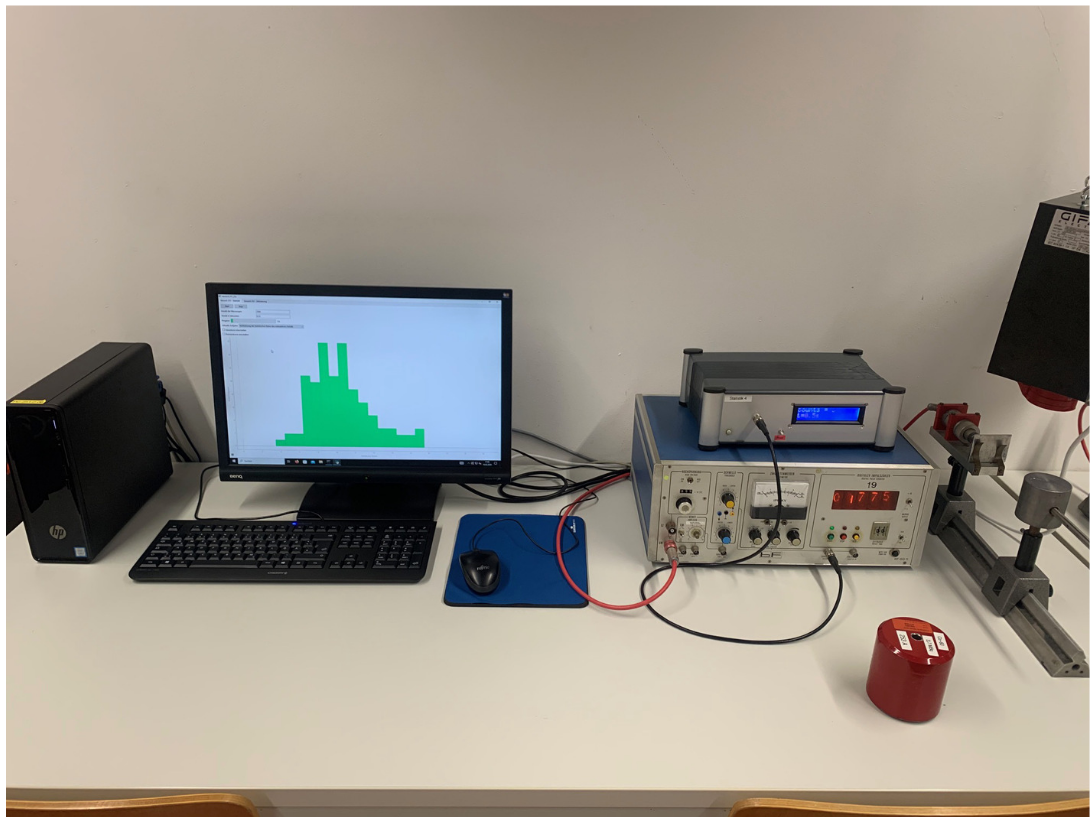
\includegraphics{graphics/aufbau.png}}
    \caption{Versuchsaufbau [Quelle: PAP2.2 Skript, S.55, Stand: 30.07.2024]}
    \label{fig:aufbau}
\end{figure}


\phantom{.}





%---------------VERSUCHSPROTOKOLL MIT MESSDATEN---------------
\newpage

\section{Versuchsprotokoll mit Messdaten}

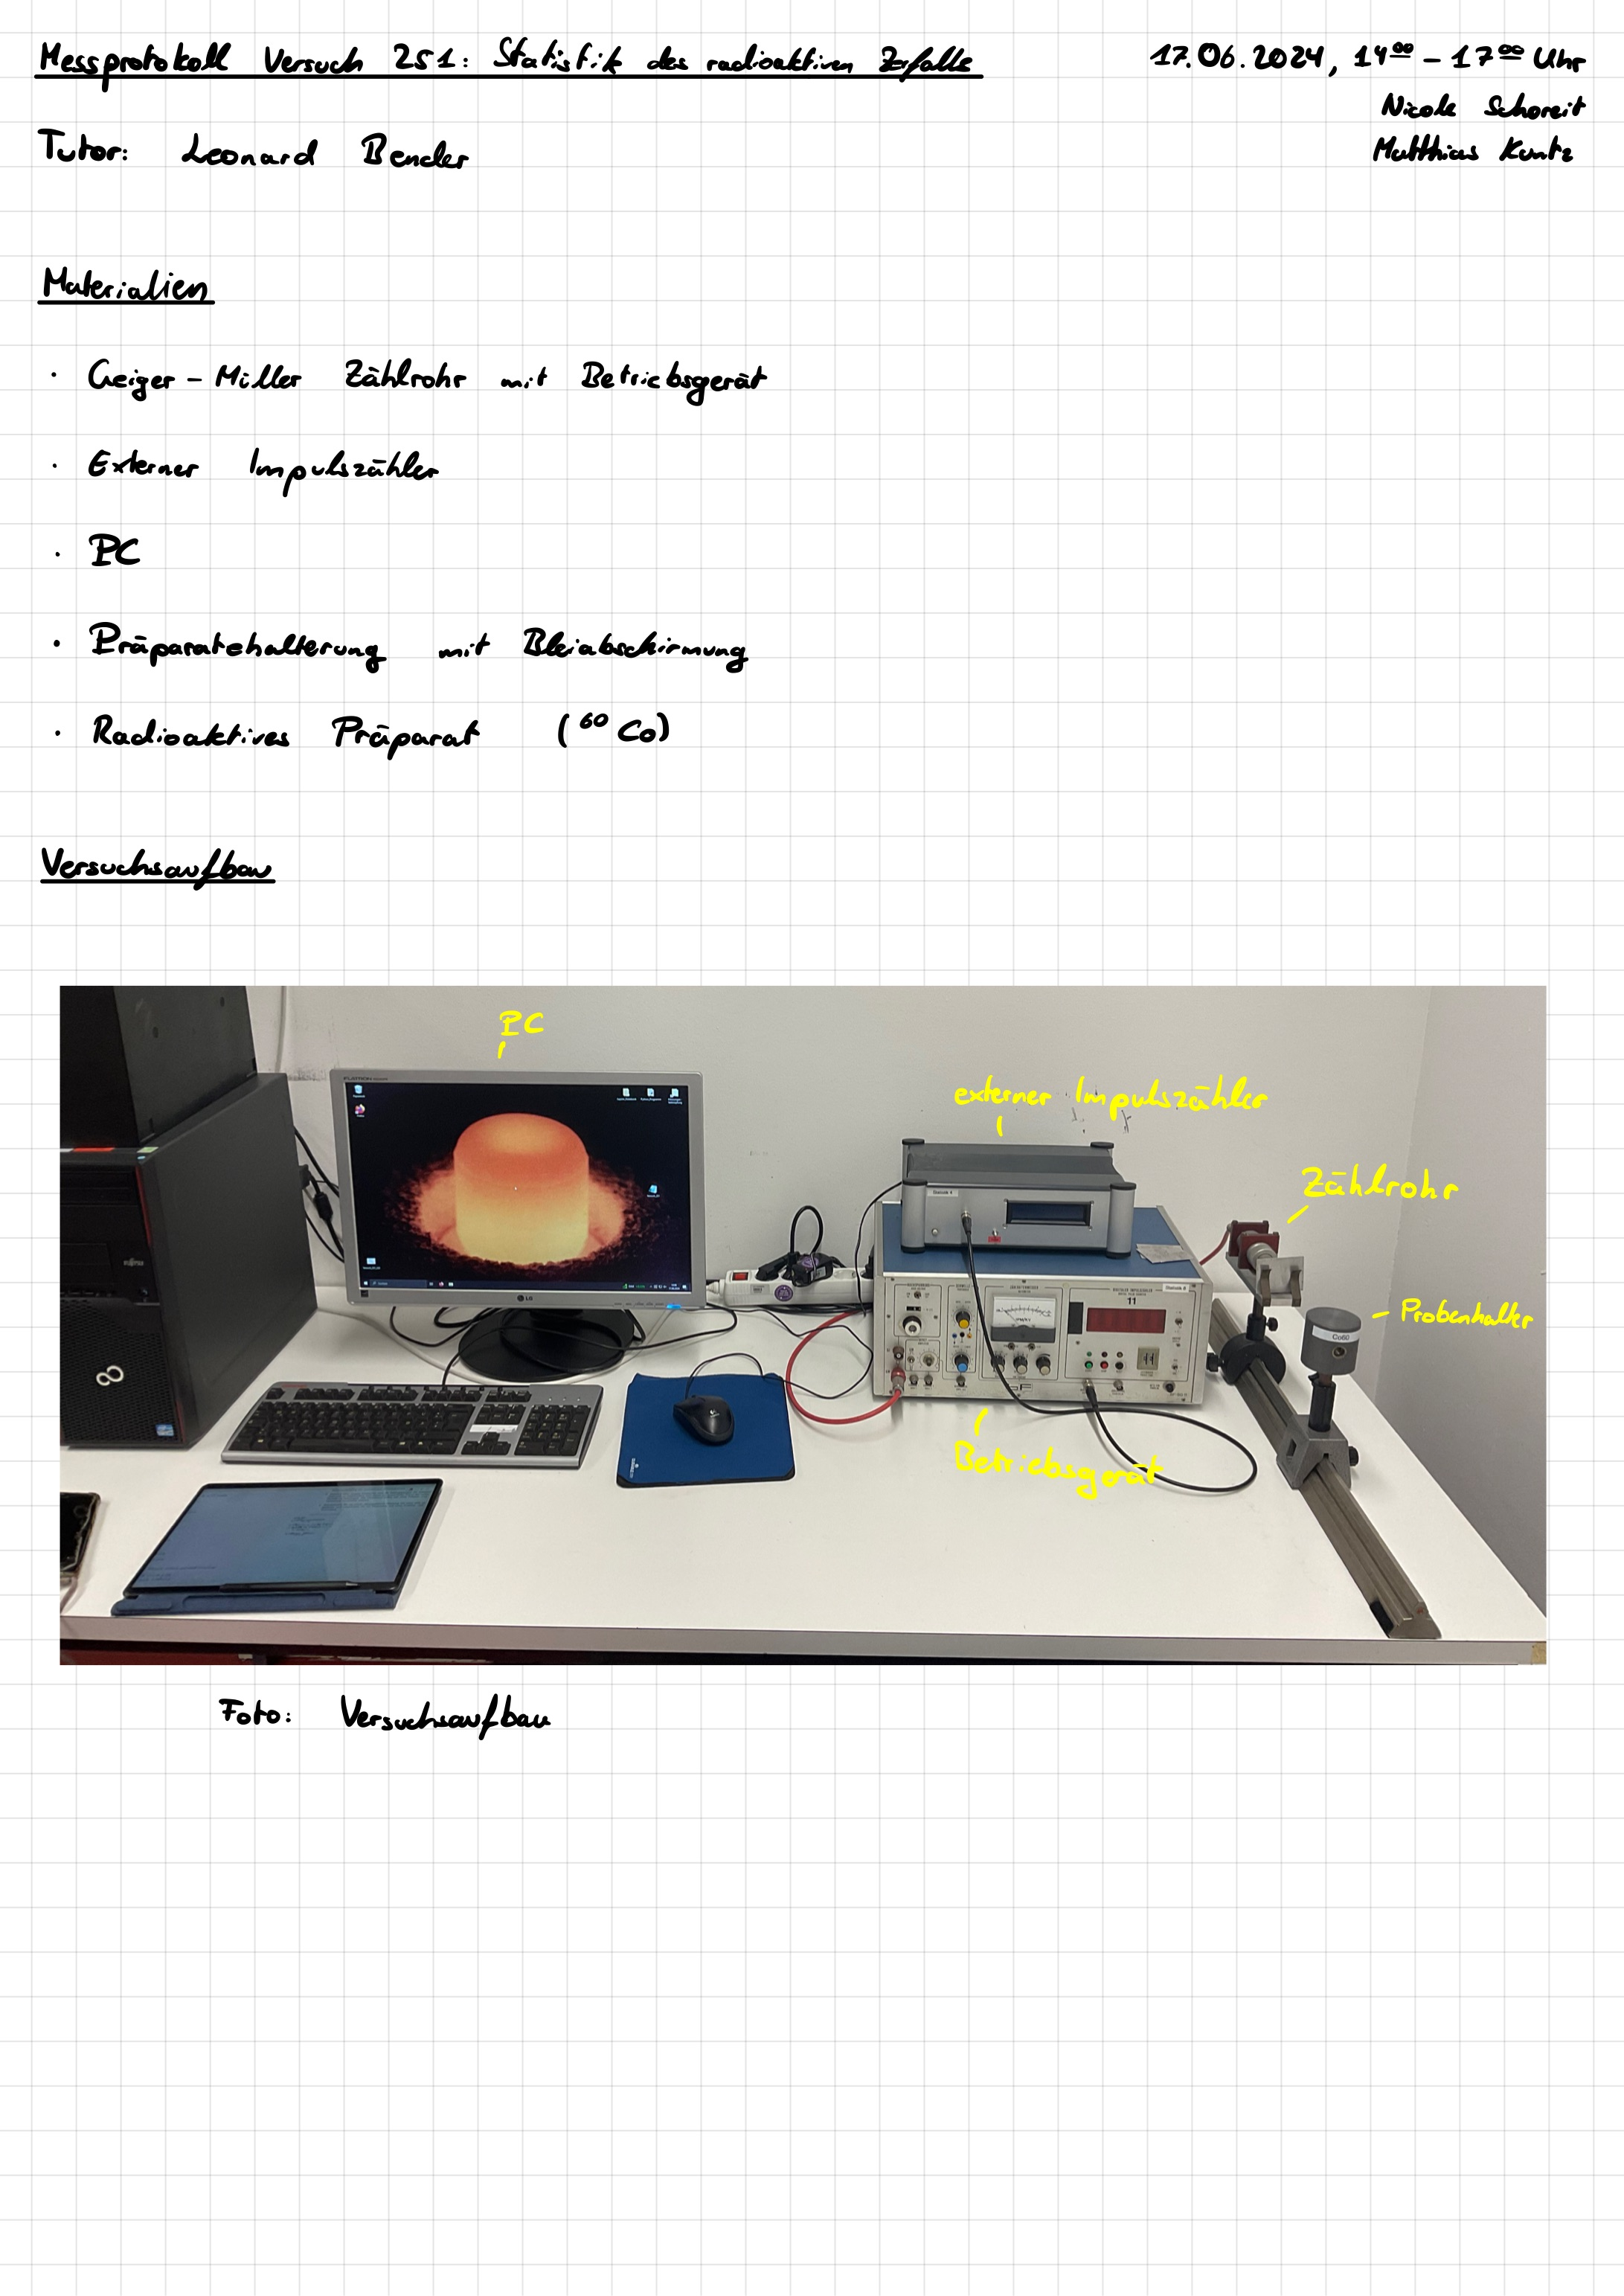
\includegraphics[width=\textwidth]{graphics/mess1.jpg}
\newpage
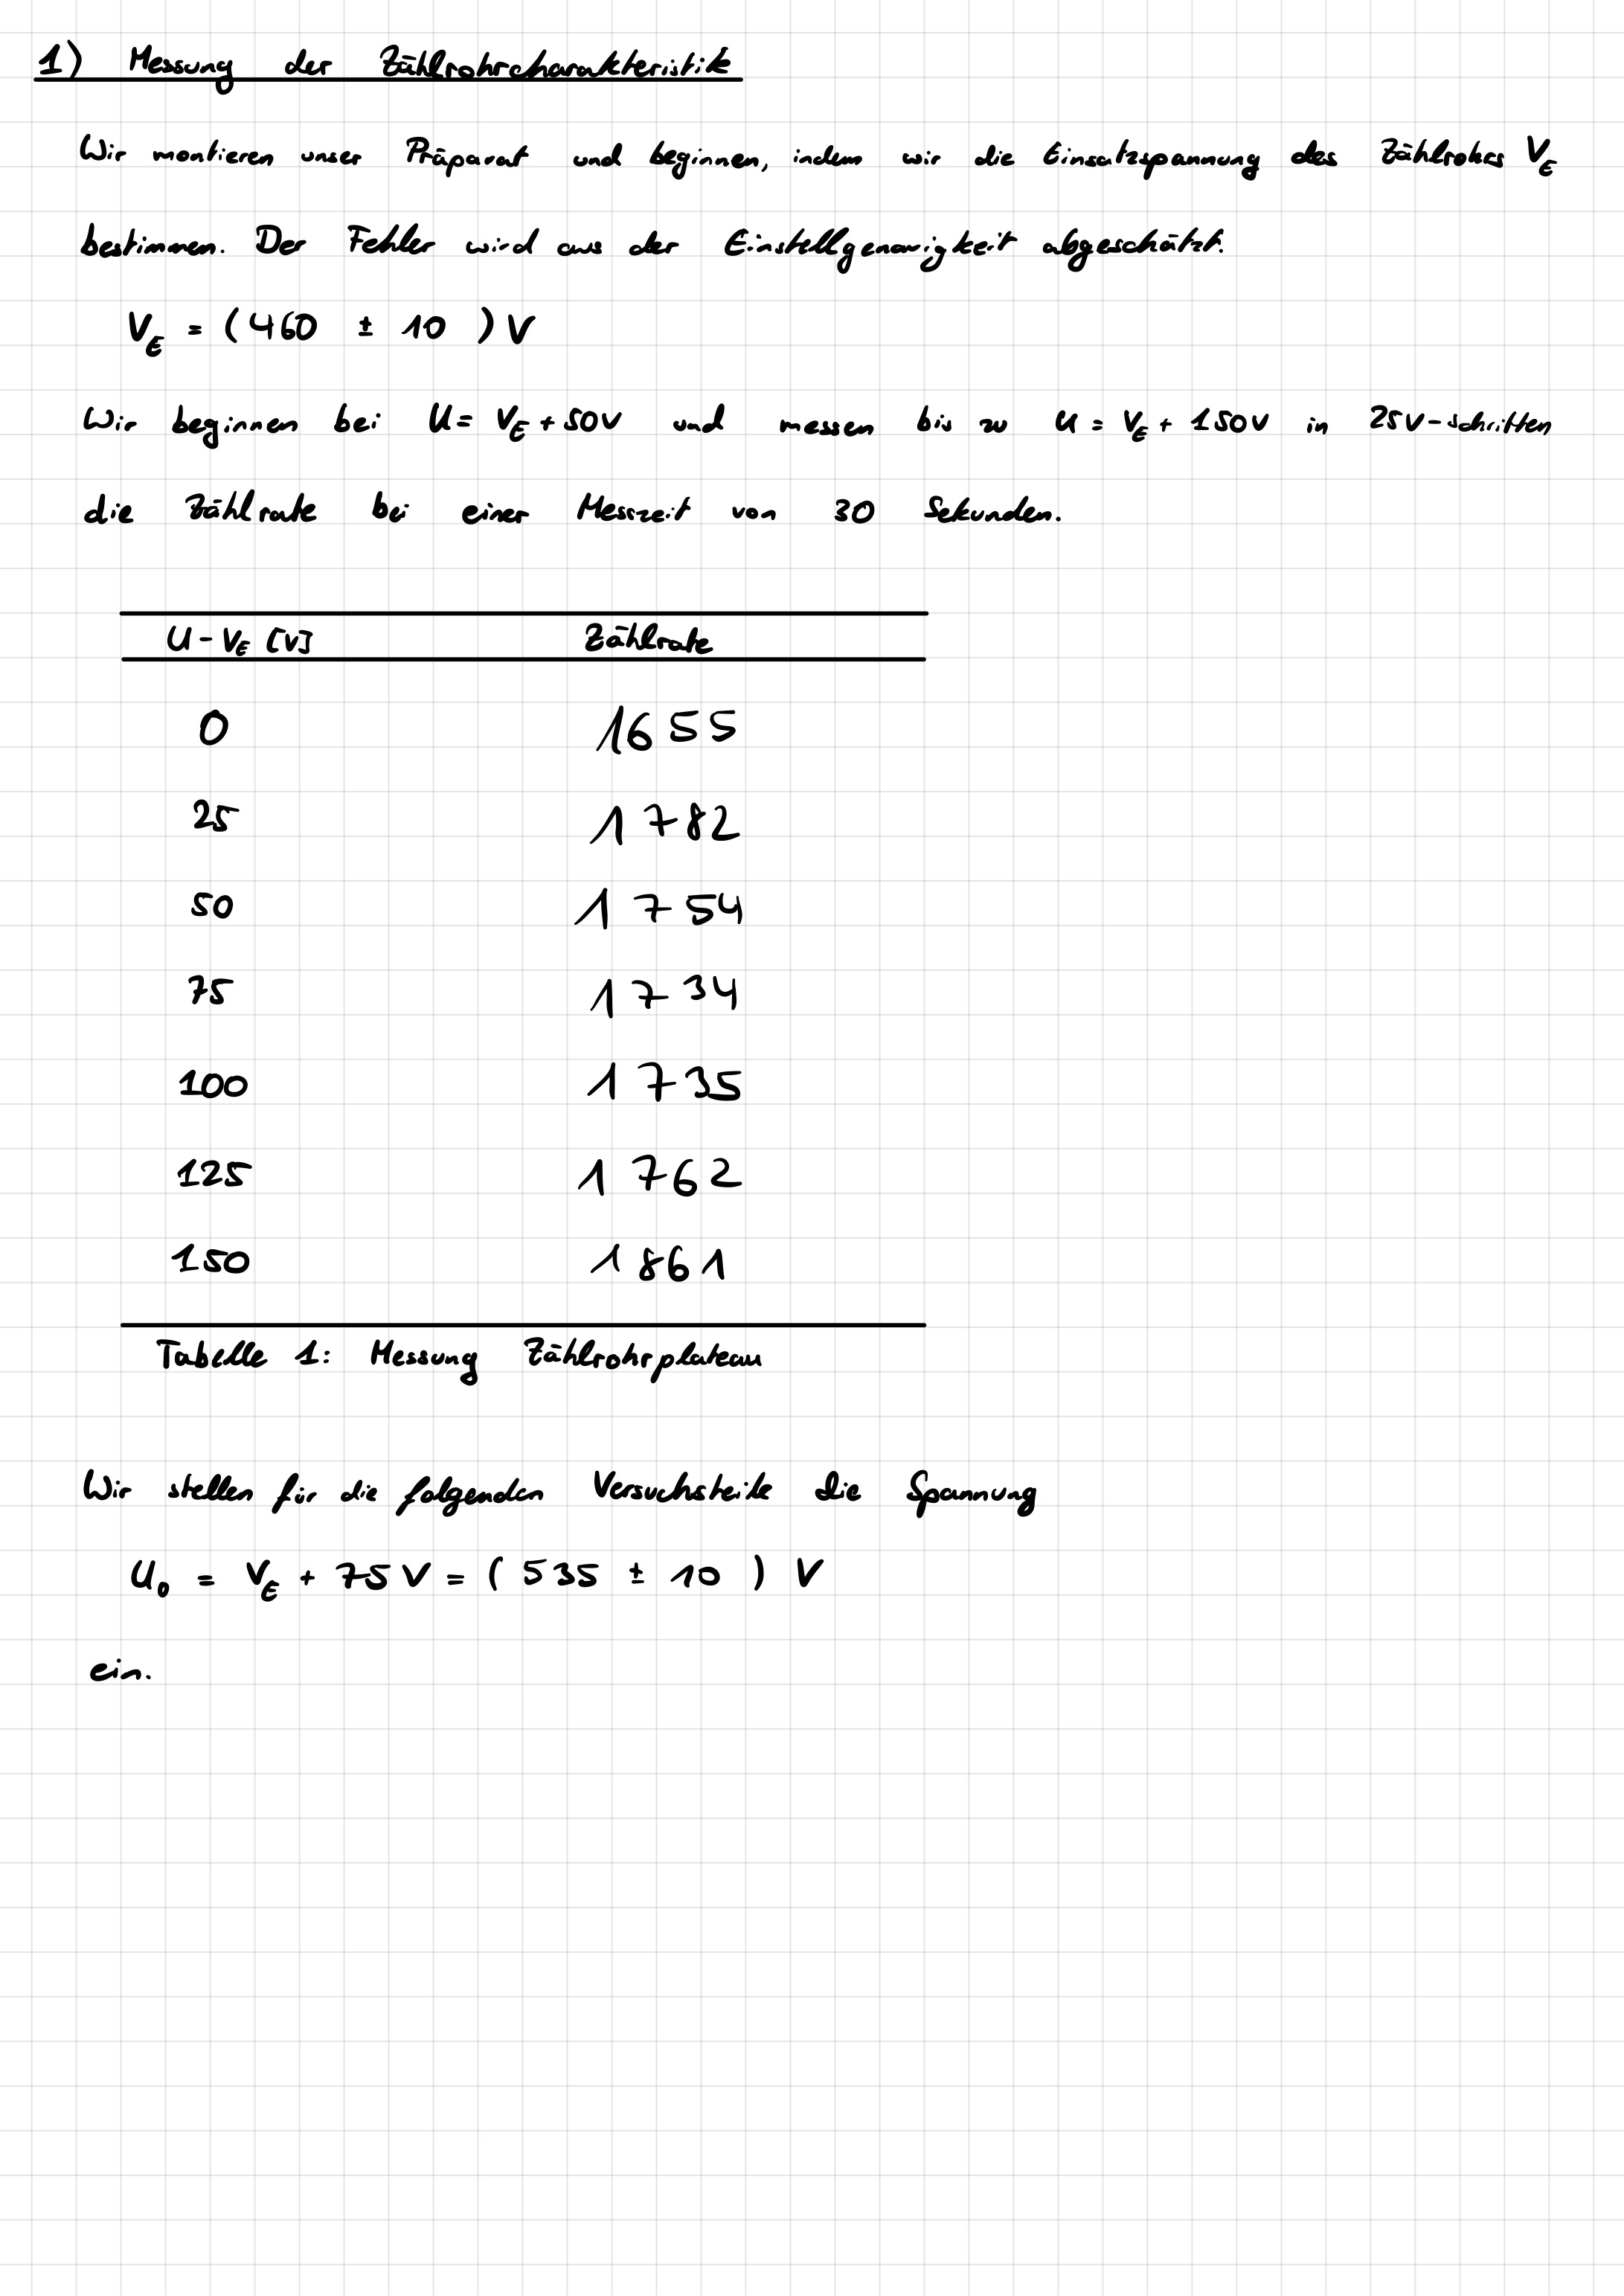
\includegraphics[width=\textwidth]{graphics/mess2.jpg}
\newpage
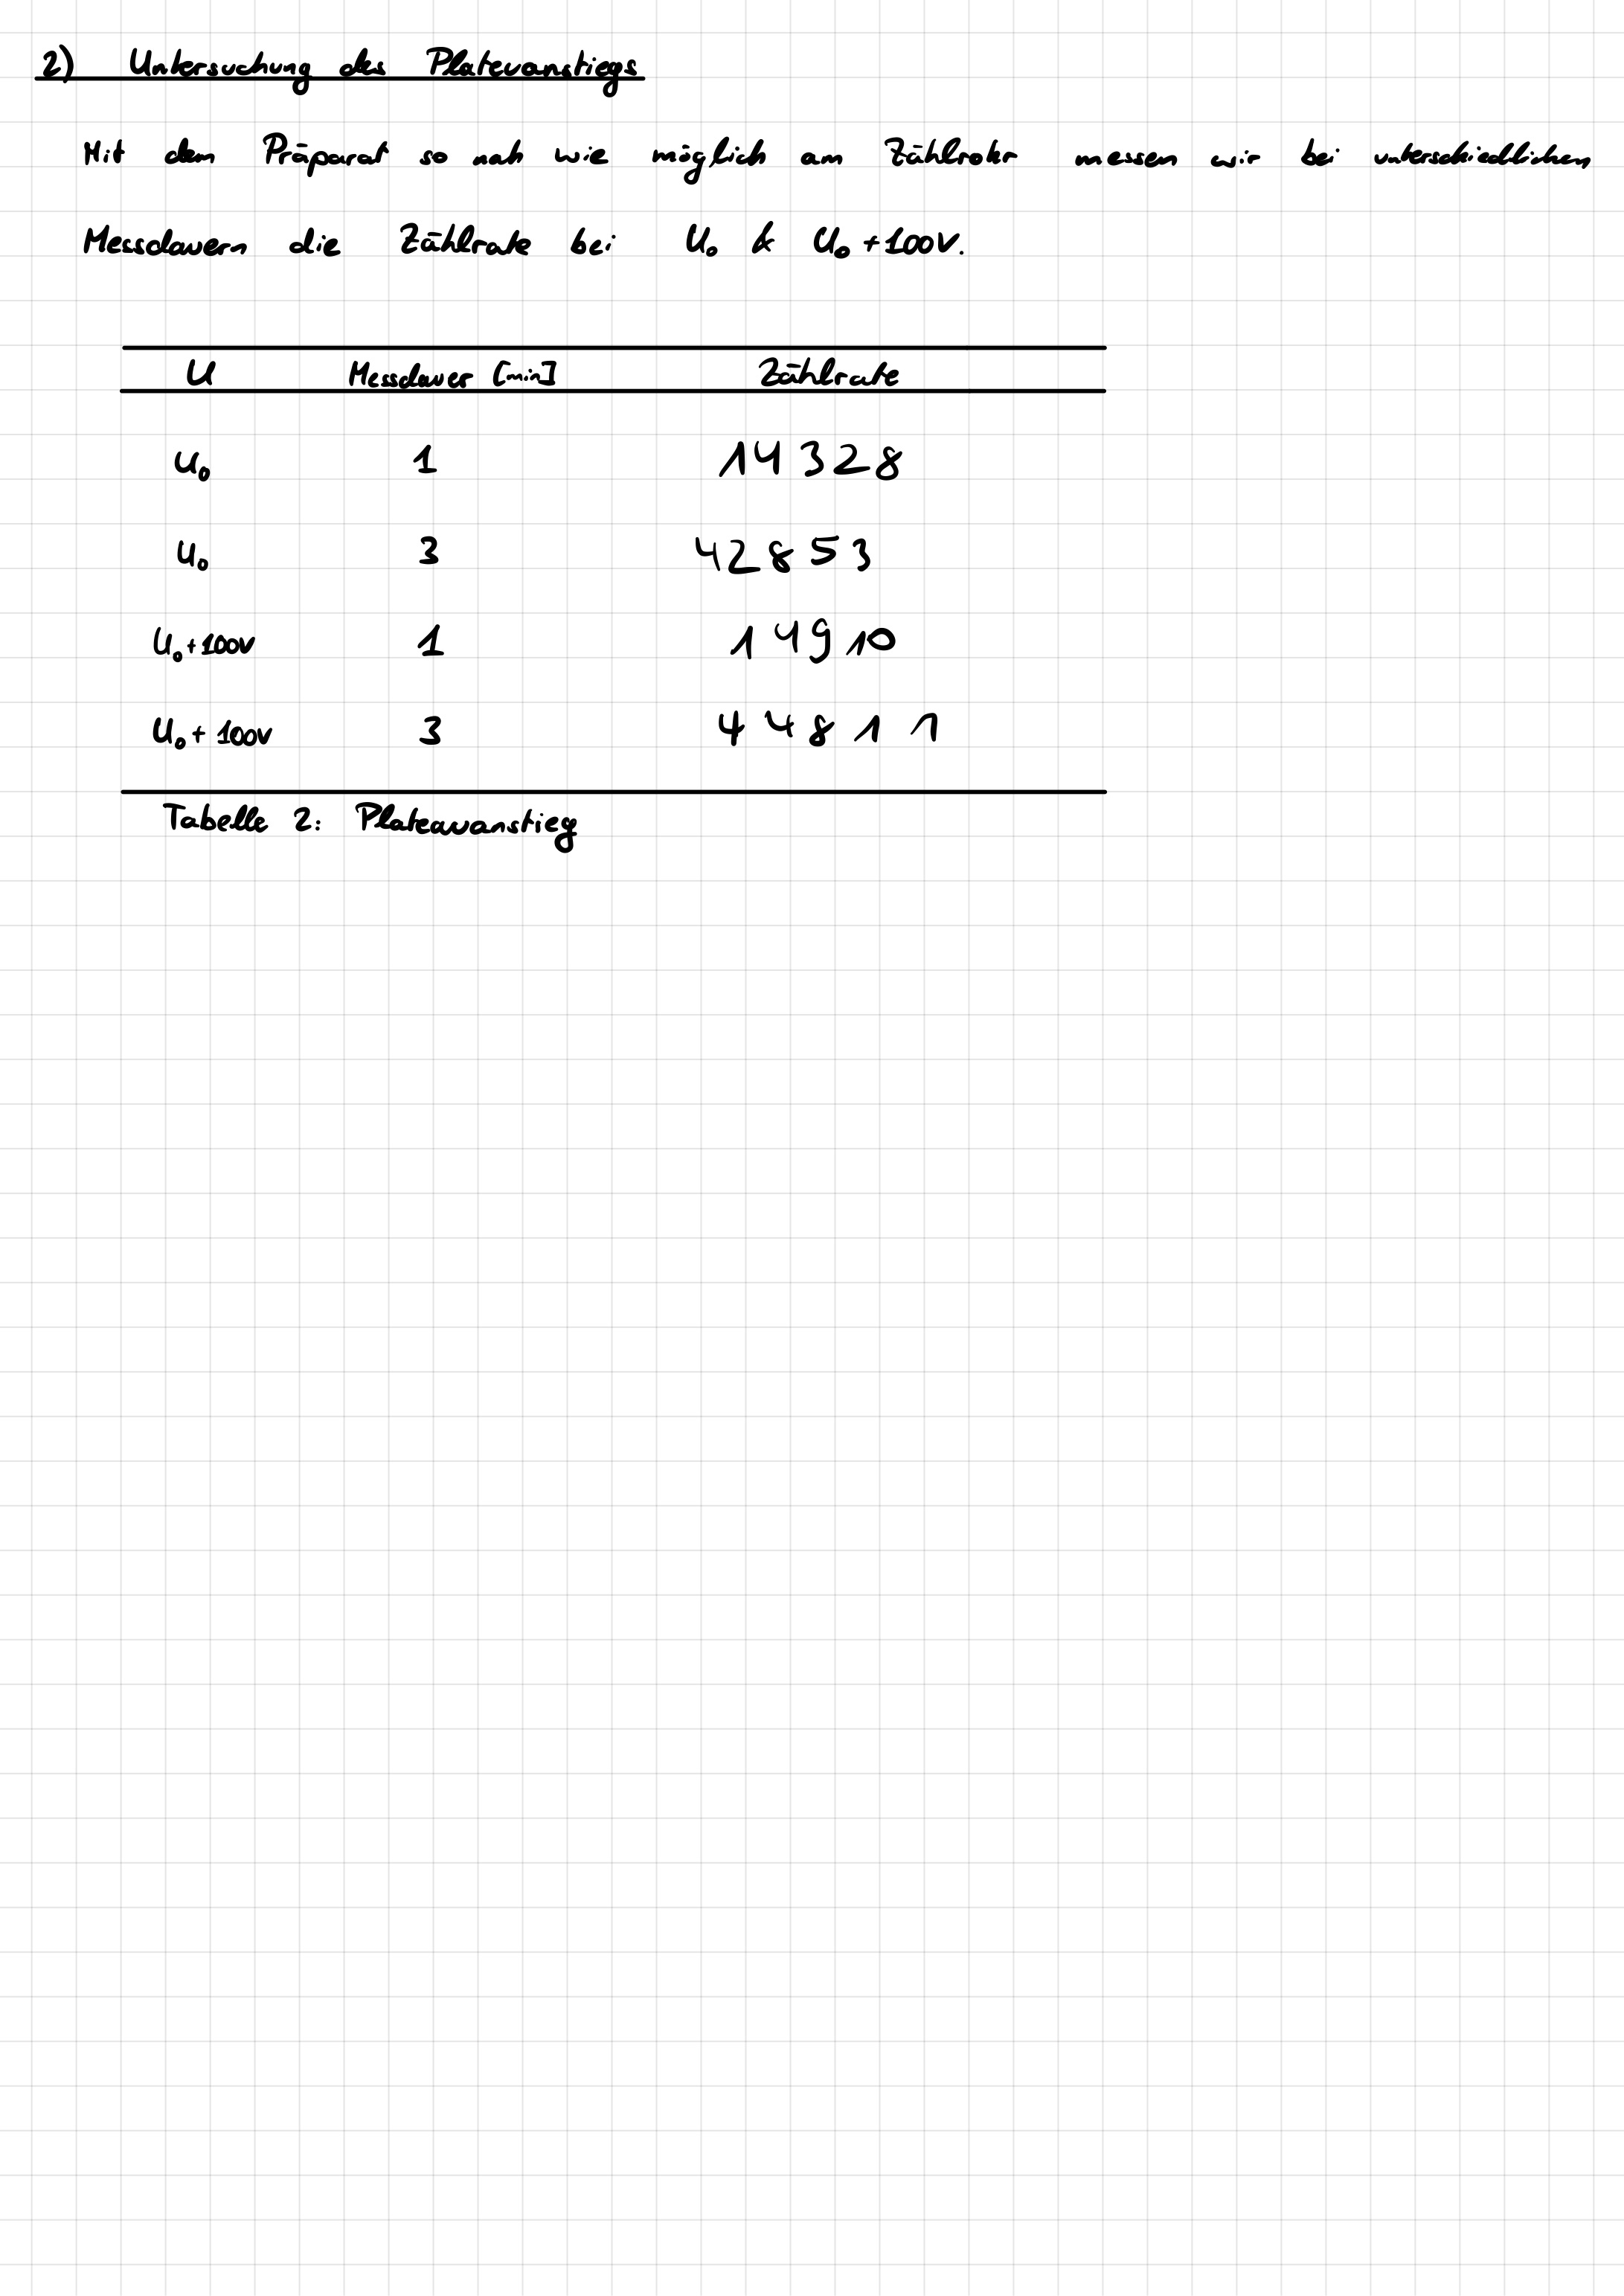
\includegraphics[width=\textwidth]{graphics/mess3.jpg}
\newpage
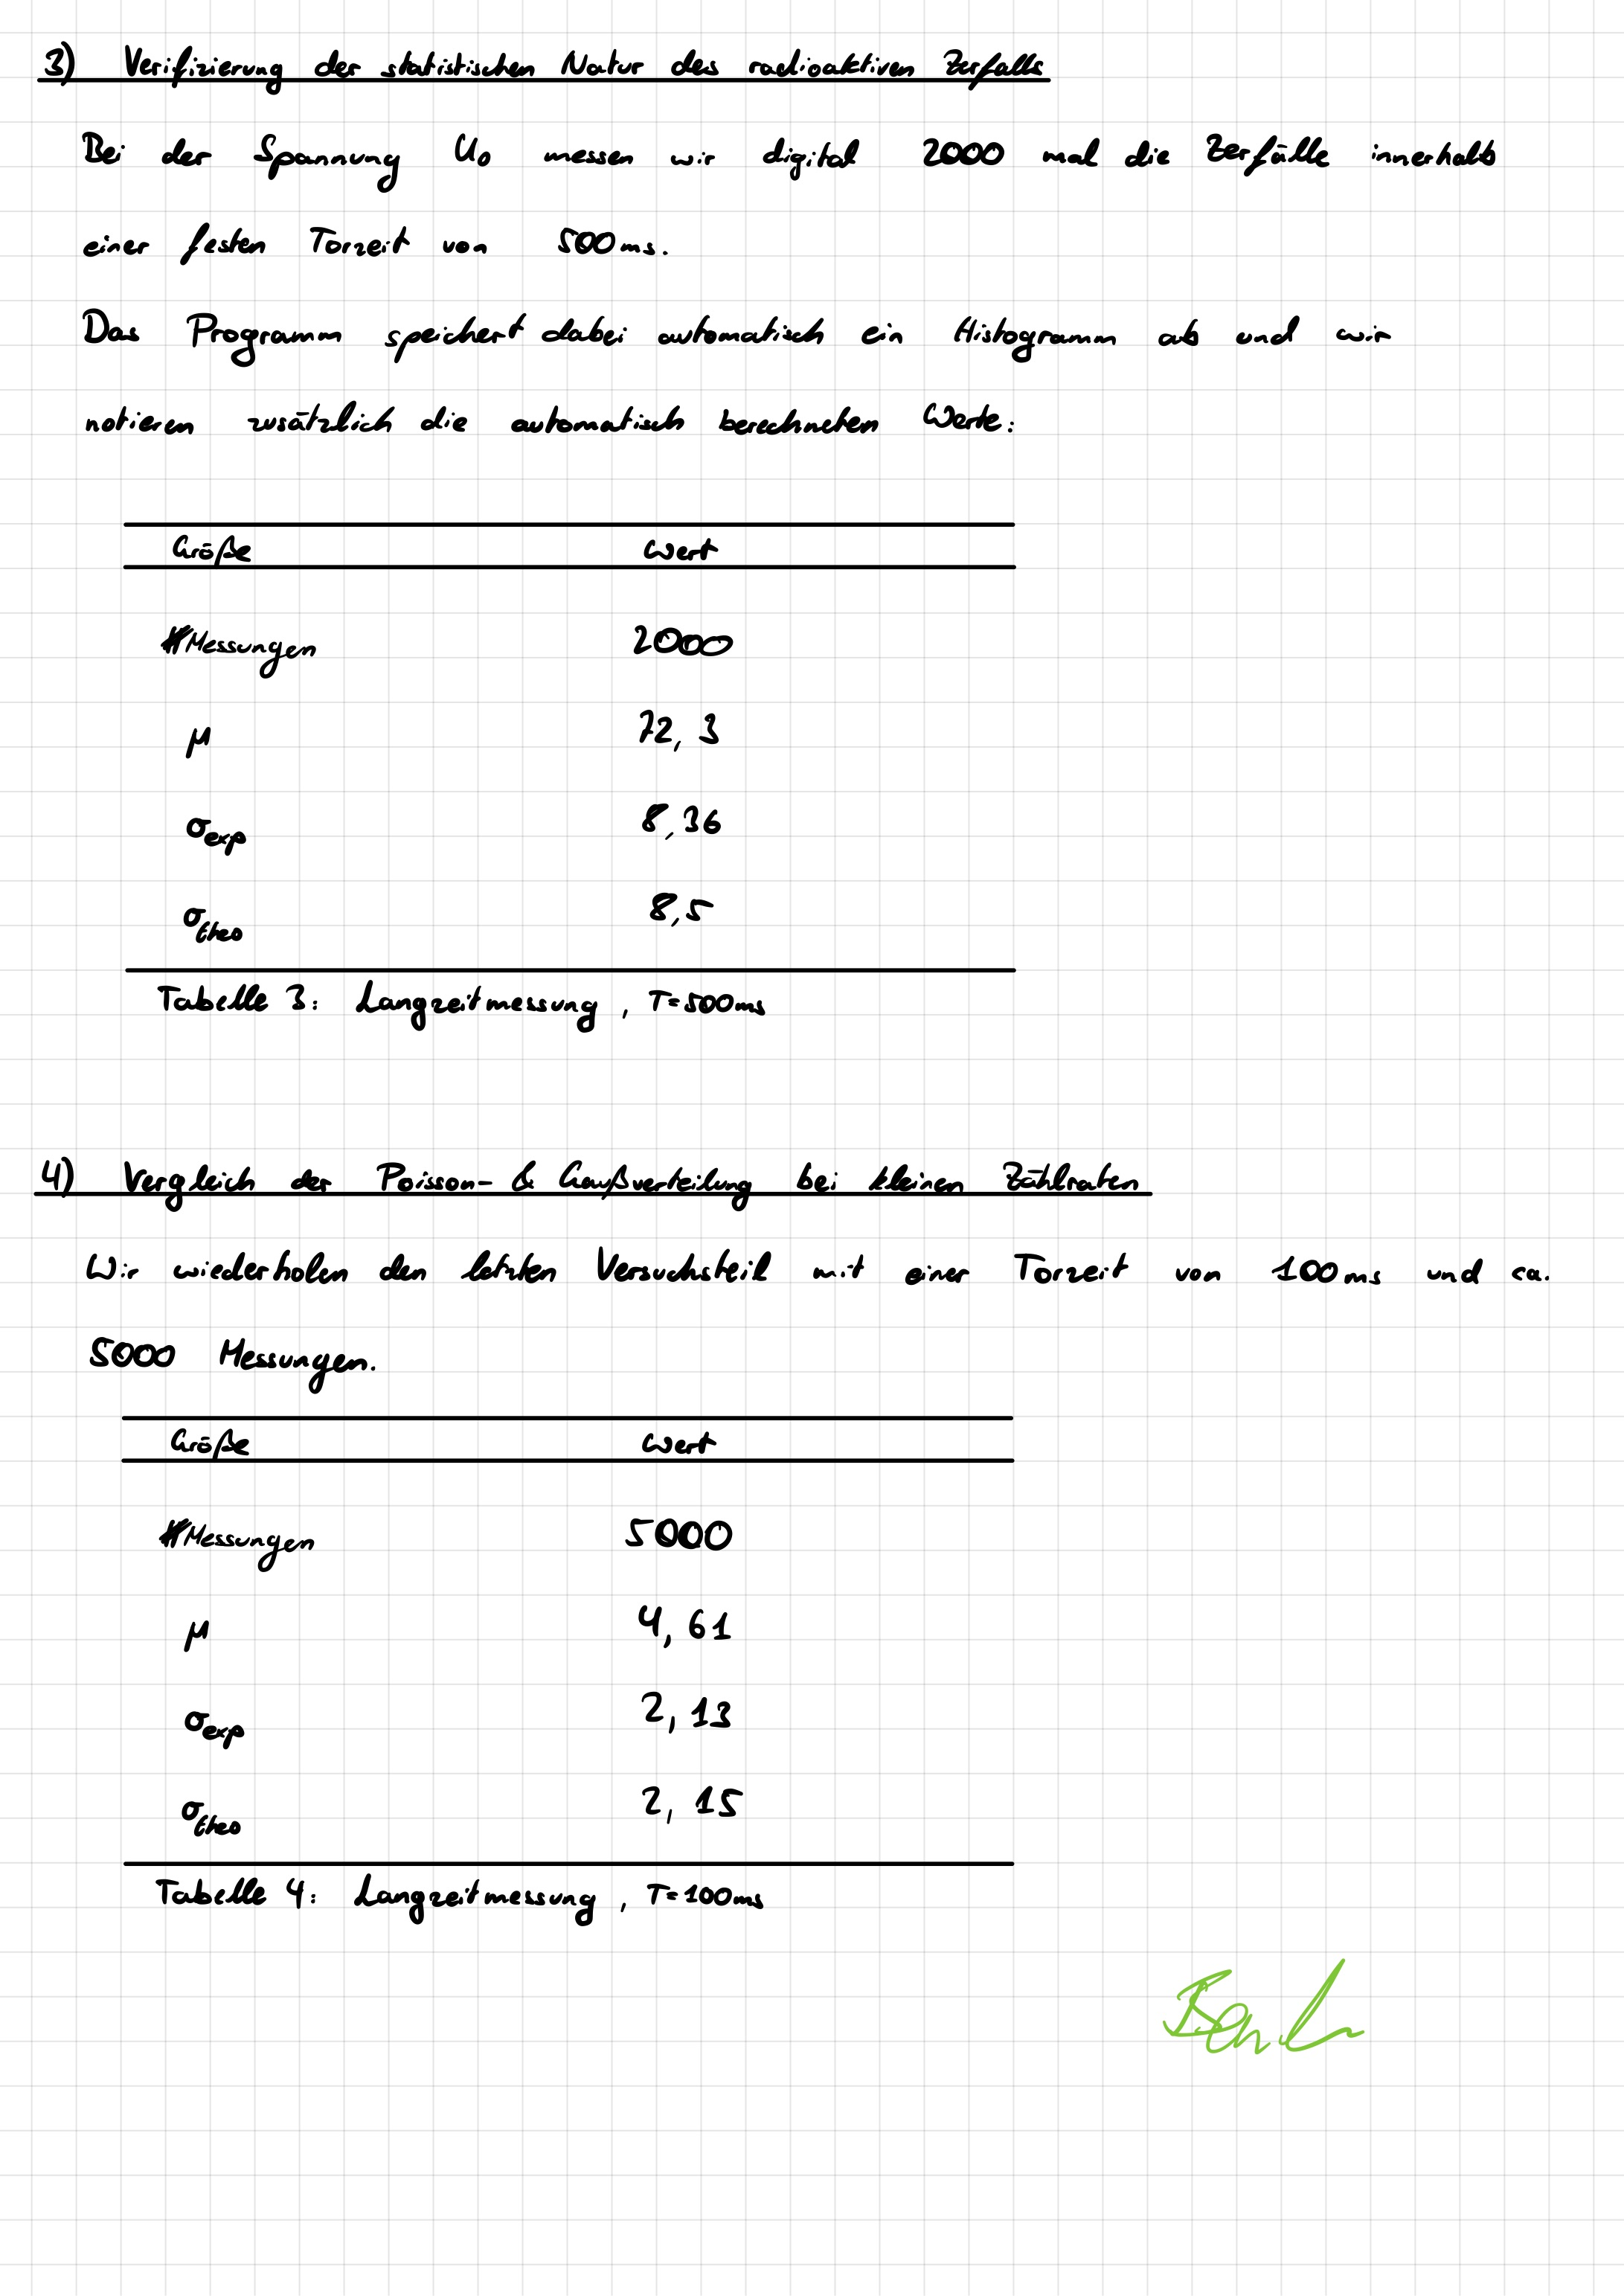
\includegraphics[width=\textwidth]{graphics/mess4.jpg}
\newpage

\addtocounter{table}{4}




\clearpage
\newpage
%-------------------------AUSWERTUNG-------------------------
\section{Auswertung}

In dieser Evaluation werden alle Fehler, sofern keine spezifische Angabe gemacht wird, mithilfe der Gauss'schen Fehlerfortpflanzung berechnet. Dies bedeutet, dass ein Wert $F$, der mit der Formel $f(a_1, ..., a_n)$ berechnet wird, den Fehler $\Delta F$ annimmt:

\begin{equation}
    \Delta F = \sqrt{\sum_n \left( \frac{\partial f}{\partial a_n} \cdot \Delta a_n \right)^2}.
\end{equation}

Des Weiteren erfolgen Signifikanztests von zwei Werten $a$ und $a'$ über die folgende Formel:

\begin{equation}
    \sigma = \frac{|a-a'|}{\sqrt{(\Delta a)^2 + (\Delta a')^2}}.
\end{equation}

Die Auswertung sowie Berechnung erfolgen über das dem Dokument angehängte Python-Programm. Hierbei erfolgen Fits von Funktionen mithilfe der 'curve\_fit'-Funktion des 'SciPy'-Packages und Plots werden mit 'matplotlib' erstellt.

Die Güte eines Fits wird mit der $\chi^2$-Summe bewertet:

\begin{equation}
    \chi^2 = \sum_i^N \left( \frac{\textit{Funktionswert}_i - \textit{Messwert}_i}{\textit{Fehler}_i} \right)^2
\end{equation}

Auch verwendet wird $\chi^2_{red} = \chi^2 / f$, wobei der Freiheitsgrad $f$ die Anzahl der Messwerte minus die Anzahl der Fitparameter ist. Der auf die Freiheitsgrade normierte Wert soll bei einem guten Fit ungefähr 1 sein.


\newpage

\subsection{Auswertung des Plateau-Bereichs}

Wir beginnen, indem wir unsere Messungen aus Tabelle 1 des Messprotokolls in ein Diagramm auftragen, wobei sich die Fehler der Zählraten $N$ gemäß $\sqrt{N}$ ergibt. An den Verlauf fitten wir eine lineare Funktion, wobei wir nur Punkte berücksichtigen, die auch im Plateau-Bereich liegen. Es ergibt sich das in Abbildung \ref{fig:A1-Plateau} dargestellte Plot. Wie gut zu erkennen ist, ist ein deutlicher Anstieg der Zählraten über dem Plateau zu erkennen und die Gerade hat eine sichtbare Steigung. Durchaus interessant ist jedoch, dass unsere Messwerte kurzzeitig abzufallen scheinen, was aber im Endeffekt auf statistische Schwankungen zurückzuführen ist.

\begin{figure}[!b]
    \centering
    \resizebox{0.9\textwidth}{!}{
    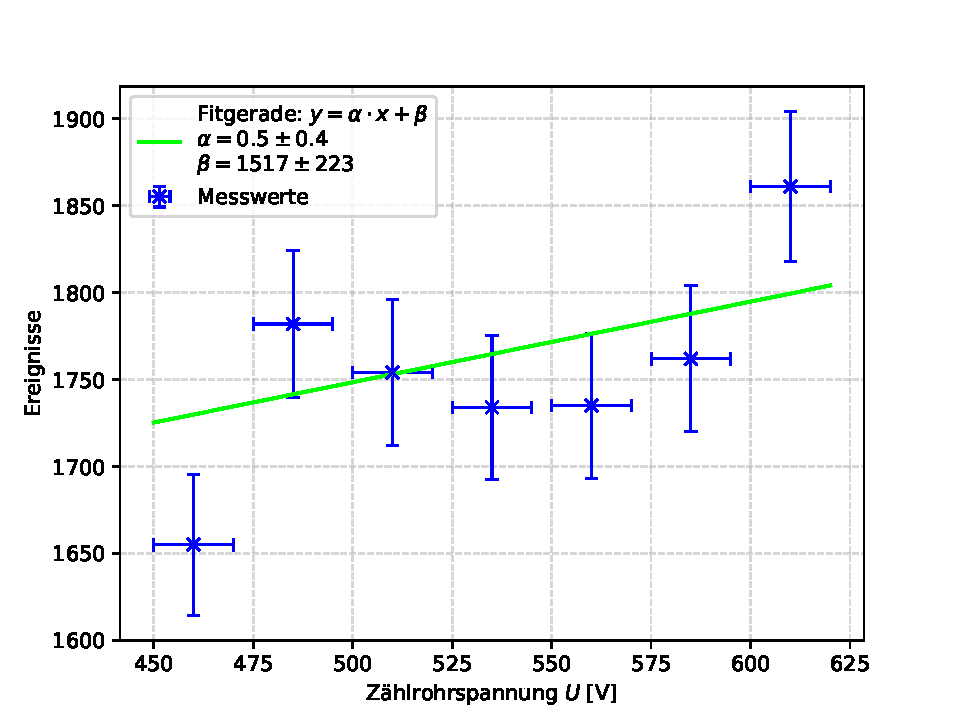
\includegraphics{plots/Plateau.pdf}}
    \caption{A1 - Plateaumessung mit Linearem Fit}
    \label{fig:A1-Plateau}
\end{figure}

Anschließend bestimmen wir aus den in Tabelle 2 aufgezeichneten Messwerten quantitativ die prozentualen Plateau-Anstiege $A$ gemäß

\begin{equation}
    \begin{split}
        A &= \frac{n(U_0 + 100V) - n(U_0)}{n(U_0)} \\
        \Rightarrow \Delta A &= A \sqrt{\left( \frac{\sqrt{\Delta n(U_0 + 100V)^2 + \Delta n(U_0)^2}}{n(U_0 + 100V) - n(U_0)} \right)^2 + \left( \frac{\Delta n(U_0)}{n(U_0)} \right)^2}
    \end{split}
\end{equation}

Die Ergebnisse für die verschiedenen Messdauern werden zusammen mit Signifikanztests in Tabelle \ref{tab:A1-ProzentualerAnstieg} eingetragen. Die Signifikanztests erfolgen zu dem theoretischen Wert einer Steigung von 0\%. 

\phantom{.}

\begin{table}[!h]
    \centering
    %\resizebox{\textwidth}{!}{
    \begin{tabular}{ccc}
        \hline
        \textbf{Messdauer} [min] & \textbf{Anstieg} [\%] & \textbf{Signifikanztest} [$\sigma$]  \\ \hline
         1 & 4,1 $\pm$ 1,2 & 3,40 \\
         3 & 4,6 $\pm$ 0,7 & 6,61 \\\hline
    \end{tabular}%}
    \caption{Prozentualer Anstieg mit Signifikanztests}
    \label{tab:A1-ProzentualerAnstieg}
\end{table}

\phantom{.}

Es ist zu erkennen, dass bei beiden Messzeiten die bestimmten Steigungen signifikant von 0 abweichen was darauf schließen lässt, dass bei einem realistischen Zählrohr wie erwartet eine nicht vernachlässigbare Steigung des Plateaus erhalten bleibt aufgrund von Inhomogenitäten des elektrischen Feldes und Nachentladungen. 

Wir möchten nun bestimmen, wie lange man messen müsste, um den Plateau-Anstieg auf 1\% genau zu kennen. Dazu betrachten wir den relativen Fehler des absoluten Anstiegs $d = n(U_0 + 100V) - n(U_0)$, wobei die Anzahl proportional zur Messzeit $t$ und somit der Fehler proportional zu $\sqrt{t}$ ist:

\begin{equation}
    \frac{\Delta d}{d} = \frac{\sqrt{\Delta n(U_0 + 100V)^2 + \Delta n(U_0)^2}}{n(U_0 + 100V) - n(U_0)} \propto \frac{\sqrt{t}}{t} = \frac{1}{\sqrt{t}}.
\end{equation}

Da nun $\Delta d / d = 0,01$ gelten soll erhalten wir den folgenden Zusammenhang mit der Messzeit $t$ einer Messung und der Gesamtmessdauer $t_{ges}$:

\begin{equation}
    \begin{split}
        \frac{\sqrt{t_{ges}}}{\sqrt{t}} &= \frac{\Delta d / d}{0,01} \\ 
        \Rightarrow t_{ges} &= \left( \frac{\Delta d / d}{0,01} \right)^2 t
    \end{split}
\end{equation}

Somit erhalten wir die in Tabelle \ref{tab:A1-Messdauern} dargestellten nötigen Gesamtmessdauern bei den gegeben Messdauern einer Einzelmessung, um den Anstieg auf 1\% Genauigkeit zu bestimmen.

\phantom{.}

\begin{table}[!h]
    \centering
    %\resizebox{\textwidth}{!}{
    \begin{tabular}{cccc}
        \hline
        \textbf{Messdauer} [min] & \textbf{rel Fehler} $\bm{\Delta d / d}$ [\%] & $\bm{t_{ges}}$ [s] & $\bm{t_{ges}}$ [h]  \\ \hline
         1 & 29,38 & 51790,84 & 14,39 \\
         3 & 15,12 & 41159,34 & 11,43 \\\hline
    \end{tabular}%}
    \caption{Benötigte Messdauern}
    \label{tab:A1-Messdauern}
\end{table}

\phantom{.}


Zuletzt betrachten wir noch die Konfidenzintervalle unserer prozentualen Steigungen, dargestellt in Tabelle \ref{tab:A1-Konfidenzintervalle}, mit den Werten für die 1-Minute Messung in der ersten und denen der 3-Minuten Messung in der zweiten Zeile. Dazu addieren beziehungsweise subtrahieren wir den Fehler beziehungsweise den doppelten Fehler von unserem Ergebnis.

\phantom{.}

\begin{table}[!h]
    \centering
    %\resizebox{\textwidth}{!}{
    \begin{tabular}{ccccc}
        \hline
        $\bm{-2\sigma}$ [\%] & $\bm{-\sigma}$ [\%] & $\bm{A}$ [\%] & $\bm{+\sigma}$ [\%] & $\bm{+2\sigma}$ [\%]  \\ \hline
        1,67 & 2,87 & 4,1 $\pm$ 1,2 & 5,26 & 6,45  \\
        3,19 & 3,88 & 4,6 $\pm$ 0,7 & 5,26 & 5,95 \\ \hline
    \end{tabular}%}
    \caption{Prozentualer Anstieg - Konfidenzintervalle}
    \label{tab:A1-Konfidenzintervalle}
\end{table}

\phantom{.}

Diese Werte sagen aus, dass bei einer Messzeit von 1 Minute etwa 68\% der gemessenen Steigungen im Bereich [2,87 , 5,26] ($1\sigma$) und ca. 95\% im Intervall [1,67 , 6,45] ($2\sigma$) liegen. Analog liegen bei einer Messzeit von 3 Minuten 68\% im Intervall [3,88 , 5,26] und 95\% im Intervall [3,19 , 5,95]. 



\newpage
\subsection{Auswertung der Messung bei großer Ereigniszahl}

Wir beginnen, indem wir die abgespeicherten Daten aus Teil 3 in Python importieren und die Häufigkeit als Funktion der Anzahl der Zerfälle pro Zeiteinheit in ein Diagramm eintragen. Dazu fitten wir an die Messwerte sowohl eine Poisson- als auch eine Gauß-Verteilung. Der resultierende Plot ist in Abbildung \ref{fig:A3-Ngroß} dargestellt. Die Parameter der Verteilungen sowie die $\chi^2$-Summen der Fits und Fit-Wahrscheinlichkeiten sind in Tabelle \ref{tab:A3-Fits} dargestellt. Der Parameter $\alpha$ steht hierbei jeweils für die Amplitude der Verteilungen.

\phantom{.}

\begin{table}[!h]
    \centering
    %\resizebox{\textwidth}{!}{
    \begin{tabular}{ccc}
        \hline
         & \textbf{Poisson} & \textbf{Gauß} \\ \hline
        $\bm{\alpha}$ [$10^{3}$] & 1,99 $\pm$ 0,05 & 1,99 $\pm$ 0,05 \\
        $\bm{\mu}$ & 72,18 $\pm$ 0,22 & 72,00 $\pm$ 0,22 \\
        $\bm{\sigma}$ & - & 8,40 $\pm$ 0,21 \\ \hline
        $\bm{\chi^2}$ & 23,55 & 24,56 \\
        $\bm{\chi^2_{red}}$ & 0,71 & 0,77 \\
        \textbf{Wsk.} & 89,0 & 82,0 \\ \hline
    \end{tabular}%}
    \caption{A3 - Fitparameter und Fitbewertung}
    \label{tab:A3-Fits}
\end{table}

\phantom{.}

\begin{figure}[!b]
    \centering
    \resizebox{0.9\textwidth}{!}{
    \includegraphics{plots/Ngroß.pdf}}
    \caption{A3 - Messung bei großer Ereigniszahl}
    \label{fig:A3-Ngroß}
\end{figure}

Sowohl am Plot als auch an den Fitparametern sowie der quantitativen Fitbewertung ist gut zu erkennen, dass beide Verteilungen innerhalb der signifikanten Stellen fast dieselben Ergebnisse liefern und ähnlich gut zu den Messwerten passen, was anhand der reduzierten $\chi^2$-Summe und der Fit-Wahrscheinlichkeit zu erkennen ist. Somit bestätigt sich, dass bei Zählstatistiken und großer Ereigniszahl die Poisson-Verteilung zur Gauß-Verteilung übergeht.

\subsection{Auswertung der Messung bei kleiner Ereigniszahl}

Wir wiederholen die soeben gemachten Schritte für die Messdaten aus Versuchsteil 4. Wir erhalten das in Abbildung dargestellte Diagramm und die in Tabelle notierten Parameter und Fitbewertungen.

\phantom{.}

\begin{table}[!h]
    \centering
    %\resizebox{\textwidth}{!}{
    \begin{tabular}{ccc}
        \hline
         & \textbf{Poisson} & \textbf{Gauß} \\ \hline
        $\bm{\alpha}$ [$10^{3}$] & 4,99 $\pm$ 0,07 & 4,94 $\pm$ 0,07 \\
        $\bm{\mu}$ & 4,62 $\pm$ 0,03 & 4,54 $\pm$ 0,03 \\
        $\bm{\sigma}$ & - & 2,108 $\pm$ 0,025 \\ \hline
        $\bm{\chi^2}$ & 7,17 & 84,42 \\
        $\bm{\chi^2_{red}}$ & 0,80 & 9,38 \\
        \textbf{Wsk.} & 62,0 & 0,0 \\ \hline
    \end{tabular}%}
    \caption{A4 - Fitparameter und Fitbewertung}
    \label{tab:A4-Fits}
\end{table}

\phantom{.}

\begin{figure}[!b]
    \centering
    \resizebox{0.9\textwidth}{!}{
    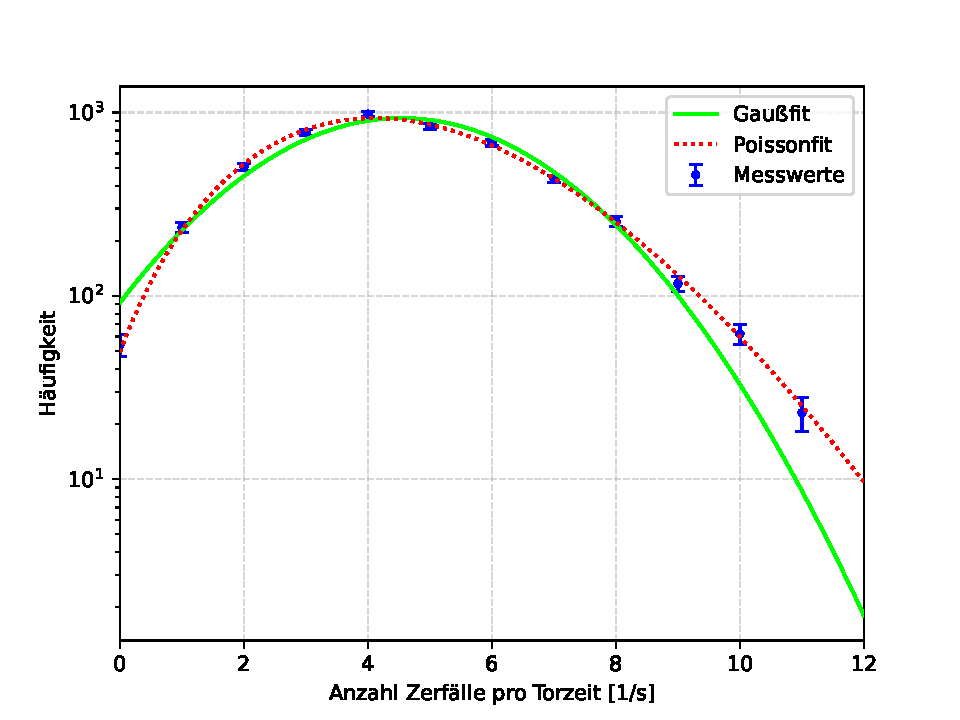
\includegraphics{plots/Nklein.pdf}}
    \caption{A4 - Messung bei kleiner Ereigniszahl}
    \label{fig:A4-Nklein}
\end{figure}

Diesmal ist deutlich zu erkennen, dass die Poisson-Verteilung deutlich besser zu den Messwerten passt als die Gauß-Verteilung. Dies ist sowohl am reduzierten $\chi^2$-Wert als auch an der Fit-Wahrscheinlichkeit des Gauß-Fits zu erkennen. Ebenso liegt der Mittelwert der Poisson-Verteilung näher an dem in Tabelle 4 notierten Mittelwert. Somit lässt sich bestätigen, dass für geringe Ereigniszahlen die asymmetrische Poisson-Verteilung akkuratere Ergebnisse liefert als die Gauß-Verteilung.



\clearpage
\newpage
%---------------PRÄSENTATION DER ENDERGEBNISSE---------------
\section{Zusammenfassung der Endergebnisse}

In diesem Versuch wurde der statistische Prozess des radioaktiven Zerfalls eines $^{60}$Co-Präparats untersucht. Dazu analysierten wir im ersten Versuchsteil die Charakteristik des verwendeten Geiger-Müller-Zählrohrs und bestimmten die prozentualen Steigungen des Plateau-Bereichs bei den Messzeiten 1 \& 3 Minuten:

\begin{equation}
    \begin{split}
        A_1 &= (4,1 \pm 1,2) \% \\
        A_3 &= (4,6 \pm 0,7) \%
    \end{split}
\end{equation}

Diese Steigungen weichen beide signifikant von 0 ab, was bestätigt, dass bei realistischen Zählrohren ein nicht zu vernachlässigender Anstieg im Plateau-Bereich bleibt.

Daraufhin bestimmten wir die benötigen Gesamtmesszeiten, um den Plateau-Anstieg auf 1\%-ige Genauigkeit zu bestimmen. Dabei erhielten wir für Einzelmessungen von 1 Minute eine Gesamtzeit von 14,39 Stunden und bei Einzelmessungen von 3 Minuten eine Zeit von 11,43 Stunden. Zuletzt wurden noch die Konfidenzintervalle der Steigungen mit den zugehörigen Wahrscheinlichkeiten einer Messung identifiziert. 

Anschließend verglichen wir die Poisson- und Gauß-Verteilung bei der Messung mit hoher Ereigniszahl. Hier konnte wie erwartet beobachtet werden, dass die beiden Verteilung fast analoge Ergebnisse liefern und die Poisson-Verteilung in die Gauß-Verteilung übergeht.

Zum Vergleich analysierten wir im letzten Schritt die Messung bei niedriger Ereigniszahl und konnten beobachten, wie die asymmetrische Poisson-Verteilung hier deutlich besser zu den Messwerten passte als die von Gauß.


\newpage
%---------------ZUSAMMENFASSUNG UND DISKUSSION---------------
\section{Diskussion}

Insgesamt konnten in diesem Versuch die gewünschten Ergebnisse und Beobachtungen erzielt werden, was an den positiven Ergebnissen in der Zusammenfassung zu sehen ist. Bei allen Versuchsteilen wurden die gewünschten Resultate erreicht und es konnten zur Theorie passende Schlüsse gezogen werden. Insbesondere der Vergleich der Gauß- und Poisson-Verteilungen in den letzten beiden Versuchsteilen lieferte aussagekräftige Ergebnisse über die Genauigkeit und Anwendbarkeit beider Verteilungen unter verschiedenen Randbedingungen. 

Ebenso konnten bei der Analyse des Plateau-Bereichs interessante Ergebnisse erzielt werden. Insbesondere der Teil über die benötigte Gesamtmessdauer zeigt, dass akkuratere Ergebnisse einen enorm viel größeren Zeitaufwand vorausgesetzt und somit den Rahmen des Physikalischen Anfängerpraktikums mehr als gesprengt hätten. 

Somit lässt sich abschließend sagen, dass in diesem Versuch durchweg positive und dem Rahmen des Praktikums angemessene Ergebnisse erzielt werden konnten, die als lehrreicher und informativer Einblick in statistische Prozesse dienen. 


 
\newpage
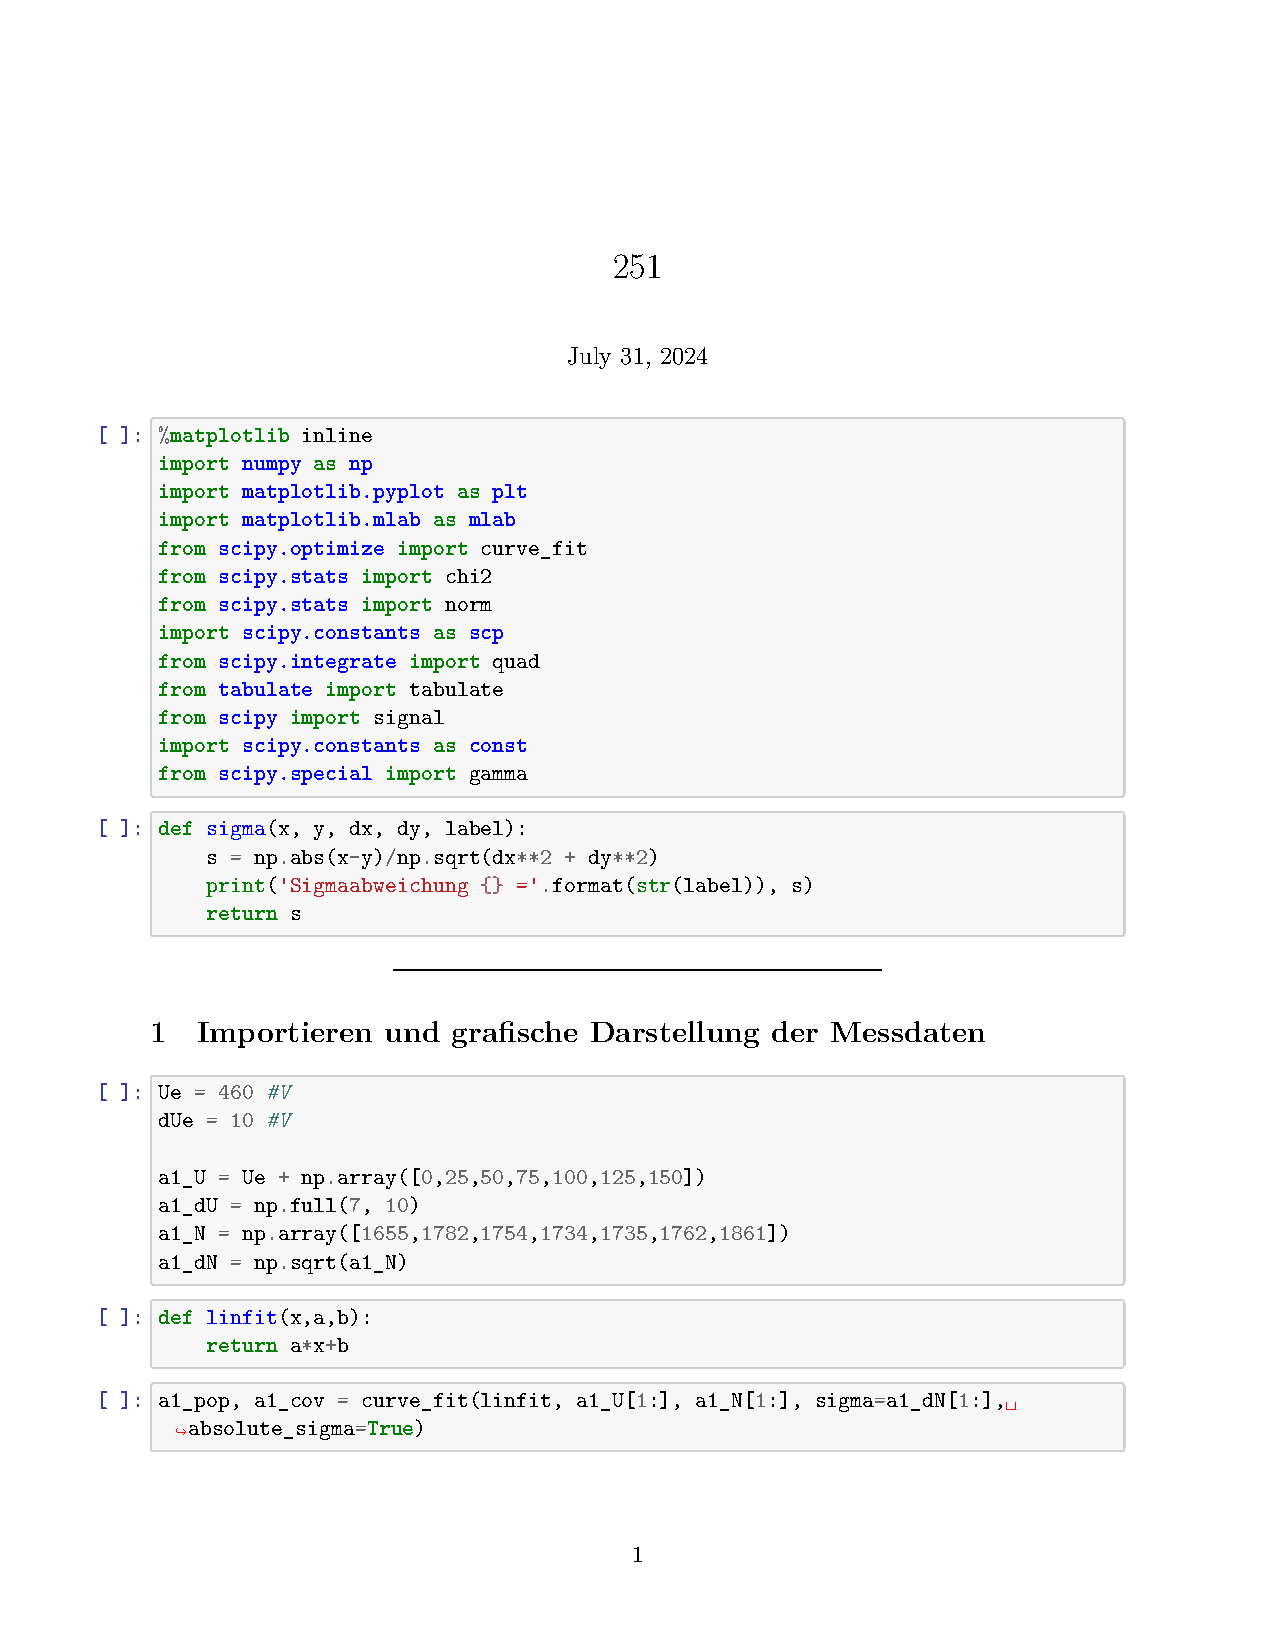
\includepdf[pagecommand=\invisiblesection{Python-Code},scale=0.8,pages=1]{251.pdf}
\includepdf[pagecommand={},scale=0.8,pages=2-last]{251.pdf}

\end{document}

